\documentclass[12pt,letterpaper]{exam}
\usepackage[lmargin=1in,rmargin=1in,tmargin=1in,bmargin=1in]{geometry}
\usepackage{../style/exams}

% -------------------
% Course & Exam Information
% -------------------
\newcommand{\course}{MAT 100: Exam 1}
\newcommand{\term}{Fall -- 2021}
\newcommand{\examdate}{10/20/2021}
\newcommand{\timelimit}{85 Minutes}

\setbool{hideans}{false} % Student: True; Instructor: False

% -------------------
% Content
% -------------------
\begin{document}

\examtitle
\instructions{Write your name on the appropriate line on the exam cover sheet. This exam contains \numpages\ pages (including this cover page) and \numquestions\ questions. Check that you have every page of the exam. Answer the questions in the spaces provided on the question sheets. Be sure to answer every part of each question and show all your work.} 
\scores
\bottomline
\newpage

% ---------
% Questions
% ---------
\begin{questions}

% Question 1
\question[8] Compute the following: \pspace
\begin{parts}
\part $4 + 4 - 5 \cdot 0 + 1 - 1= 4 + 4 - 0 + 1 - 1= 8$ \vfill
\part $12/4 \cdot 3 - 1= 3 \cdot 3 - 1= 9 - 1= 8$ \vfill
\part $-5 - 6 + 2 \cdot 3^2= -5 - 6 + 2 \cdot 9= -5 - 6 + 18= 7$ \vfill
\part $10/5 - 6(3 - 4)^3= 10/5 - 6(-1)^3= 10/5 - 6(-1)= 2 + 6= 8$ \vfill
\end{parts}



\newpage



% Question 2
\question[8] Simplify the following, being sure to have no negative exponents in your expression. \pspace
\begin{parts}
\part $\dfrac{x^{-6}}{x^{-3}}= \dfrac{x^3}{x^6}= \dfrac{1}{x^3}$ \vfill
\part $\dfrac{(xy^2)^2}{x^2 y^3}= \dfrac{x^2 y^4}{x^2y^3}= y$ \vfill
\part $\dfrac{x^6 y^{-3}}{x^3 y^2}= \dfrac{x^6}{x^3y^2y^3}= \dfrac{x^3}{y^5}$ \vfill
\part $\left( \dfrac{y^3}{x^2} \right)^{-2}= \left( \dfrac{x^2}{y^3} \right)^{2}= \dfrac{x^4}{y^6}$ \vfill
\end{parts}



\newpage



% Question 3
\question[8] Compute the following, being sure to simplify your answer completely: \pspace
\begin{parts}
\part $4 + \dfrac{1}{5}= \dfrac{20}{5} + \dfrac{1}{5}= \dfrac{21}{5}$ \vfill
\part $\dfrac{3}{10} - \dfrac{5}{4}= \dfrac{6}{20} - \dfrac{25}{20}= \dfrac{6 - 25}{20}= -\dfrac{19}{20}$ \vfill
\part $\dfrac{6}{35} \cdot \dfrac{7}{15}= \dfrac{2}{5} \cdot \dfrac{1}{5}= \dfrac{2}{25}$ \vfill
\part $\dfrac{-\frac{7}{5}\phantom{-}}{\frac{21}{10}}= -\dfrac{7}{5} \cdot \dfrac{10}{21}= -\dfrac{1}{1} \cdot \dfrac{2}{3}= -\dfrac{2}{3}$ \vfill
\end{parts}



\newpage



% Question 4
\question[6] Write a mathematical expression that computes the following: \pspace
\begin{parts}
\item 33\% of 48 \hspace{4.5cm} $48(0.33)$ \vfill
\item 92\% of 172 \hspace{4.2cm} $172(0.92)$ \vfill
\item 121\% of 16 \hspace{4.2cm} $16(1.21)$ \vfill
\end{parts} \vfill



% Question 5
\question[6] Write a mathematical expression that computes the following: \pspace
\begin{parts}
\item 71 decreased by 90\% \hspace{2.7cm} $71(1 - 0.90)= 71(0.10)$ \vfill
\item 88 increased by 30\% \hspace{2.8cm} $88(1 + 0.30)= 88(1.30)$ \vfill
\item 55 increased by 190\% \hspace{2.5cm} $55(1 + 1.90)= 55(2.90)$ \vfill
\end{parts}



\newpage



% Question 6
\question[4] Convert the following decimal numbers to scientific notation: \pspace
\begin{parts}
\part $7400= 7.4 \cdot 10^3$ \vfill
\part $0.002= 2.0 \cdot 10^{-3}$ \vfill
\end{parts} \vfill



% Question 7
\question[4] Convert the following numbers in scientific notation to decimal notation: \pspace
\begin{parts}
\part $8.0 \cdot 10^{-6}= 0.000008$ \vfill
\part $1.65 \cdot 10^3= 1650$ \vfill
\end{parts}



\newpage



% Question 8
\question[6] Find the prime factorizations of the following integers: \pspace
\begin{parts}
\part $210= 2 \cdot 3 \cdot 5 \cdot 7$ \vfill
\part $125= 5^3$ \vfill
\part $88= 2^3 \cdot 11$ \vfill
\end{parts}



% Question 9
\question[8] Compute the following: \pspace
\begin{parts}
\part $\gcd(14,21)= \gcd(2 \cdot 7, 3 \cdot 7)= 7$ \vfill
\part $\lcm(6,20)= \lcm(2 \cdot 3, 2^2 \cdot 5)= 2^2 \cdot 3 \cdot 5= 60$ \vfill
\part $\gcd(252, 9720)= \gcd(2^2 \cdot 3^2 \cdot 7, 2^3 \cdot 3^5 \cdot 5)= 2^2 \cdot 3^2$ \vfill
\part $\lcm(252, 9720)= \lcm(2^2 \cdot 3^2 \cdot 7, 2^3 \cdot 3^5 \cdot 5)= 2^3 \cdot 3^5 \cdot 5 \cdot 7$ \vfill
\end{parts}



\newpage



% Question 10
\question[6] Simplify the following as much as possible: \pspace
\begin{parts} 
\part $\sqrt{50}= \sqrt{2 \cdot 5^2}= 5 \sqrt{2}$ \vfill
\part $\sqrt{80}= \sqrt{2^4 \cdot 5}= 2^2 \sqrt{5}= 4 \sqrt{5}$ \vfill
\part $\sqrt[3]{2^2 \cdot 3^6 \cdot 5}= 3^2 \sqrt[3]{2^2 \cdot 5}= 9 \sqrt[3]{4 \cdot 5}= 9 \sqrt[3]{20}$ \vfill
\end{parts}



\newpage



% Question 11
\question[6] Consider the following relations below:

	\[
	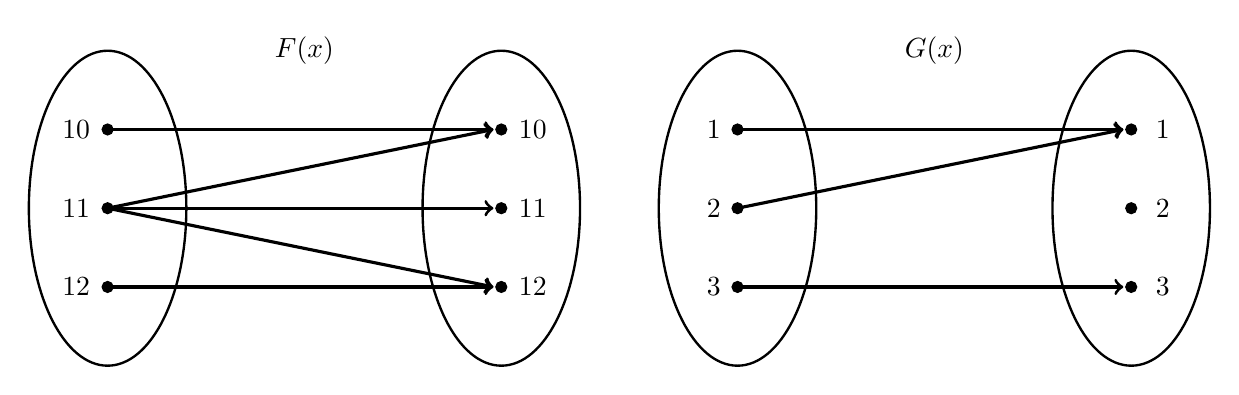
\begin{tikzpicture}
	\node at (2.5,2) {$F(x)$};
	
	% Ellipses
	\draw[line width=0.03cm] (0,0) circle (1 and 2);
	\draw[line width=0.03cm] (5,0) circle (1 and 2);
	
	% Nodes
	\draw[fill=black] (0,1) circle (0.07);
	\draw[fill=black] (0,0) circle (0.07);
	\draw[fill=black] (0,-1) circle (0.07);
	
	\draw[fill=black] (5,1) circle (0.07);
	\draw[fill=black] (5,0) circle (0.07);
	\draw[fill=black] (5,-1) circle (0.07);
	
	% Arrow
	\draw[line width=0.04cm,->] (0,1) -- (4.9,1);
	\draw[line width=0.04cm,->] (0,0) -- (4.9,1);
	\draw[line width=0.04cm,->] (0,0) -- (4.9,0);
	\draw[line width=0.04cm,->] (0,0) -- (4.9,-1);
	\draw[line width=0.04cm,->] (0,-1) -- (4.9,-1);
	
	% Labels
	\node at (-0.4,1) {$10$};
	\node at (-0.4,0) {$11$};
	\node at (-0.4,-1) {$12$};
	
	\node at (5.4,1) {$10$};
	\node at (5.4,0) {$11$};
	\node at (5.4,-1) {$12$};
	
	%
	\tikzset{shift={(8,0)}}	
	
	\node at (2.5,2) {$G(x)$};
	
	% Ellipses
	\draw[line width=0.03cm] (0,0) circle (1 and 2);
	\draw[line width=0.03cm] (5,0) circle (1 and 2);
	
	% Nodes
	\draw[fill=black] (0,1) circle (0.07);
	\draw[fill=black] (0,0) circle (0.07);
	\draw[fill=black] (0,-1) circle (0.07);
	
	\draw[fill=black] (5,1) circle (0.07);
	\draw[fill=black] (5,0) circle (0.07);
	\draw[fill=black] (5,-1) circle (0.07);
	
	% Arrow
	\draw[line width=0.04cm,->] (0,1) -- (4.9,1);
	\draw[line width=0.04cm,->] (0,0) -- (4.9,1);
	\draw[line width=0.04cm,->] (0,-1) -- (4.9,-1);
	
	% Labels
	\node at (-0.3,1) {$1$};
	\node at (-0.3,0) {$2$};
	\node at (-0.3,-1) {$3$};
	
	\node at (5.4,1) {$1$};
	\node at (5.4,0) {$2$};
	\node at (5.4,-1) {$3$};
	\end{tikzpicture}
	\] \pspace

	\begin{minipage}[b]{0.49\textwidth}
	\centering
	\begin{tabular}{c|rcc|r}
	$x$ & $H(x)$ & \hspace{1cm} & $x$ & $J(x)$ \\ \cline{1-2} \cline{4-5}
	$1$ & $1$ & & $5$ & $-1$ \\
	$2$ & $2$ & & $6$ & $-2$ \\
	$3$ & $3$ & & $7$ & $-3$ \\
	$4$ & $4$ & & $8$ & $-4$ \\
	$1$ & $5$ & & $9$ & $-6$
	\end{tabular}
	\end{minipage}
	\begin{minipage}[b]{0.49\textwidth}
	\[
	\begin{aligned}
	K(x)&:= 0.782x - 1283 \\[0.6cm]
	L(x)&:= 2x(x^2 + 1)(x^4 + 1)
	\end{aligned}
	\]
	\end{minipage} \pvspace{0.6cm}
	
Determine if each of the relations given above is a function. If the relation is a function, write `T' (True) and if the relation is \emph{not} a function, write `F' (False): \pspace

	\begin{enumerate}[(a)]
	\item \usol{0.66cm}{\itshape F}: $F(x)$ \pvspace{0.3cm}
	\item \usol{0.65cm}{\itshape T}: $G(x)$ \pvspace{0.3cm}
	\item \usol{0.66cm}{\itshape F}: $H(x)$ \pvspace{0.3cm}
	\item \usol{0.65cm}{\itshape T}: $J(x)$ \pvspace{0.3cm}
	\item \usol{0.65cm}{\itshape T}: $K(x)$ \pvspace{0.3cm}
	\item \usol{0.65cm}{\itshape T}: $L(x)$
	\end{enumerate}



\newpage



% Question 12
\question[4] Consider the relation plotted below.
	\[
	\fbox{
	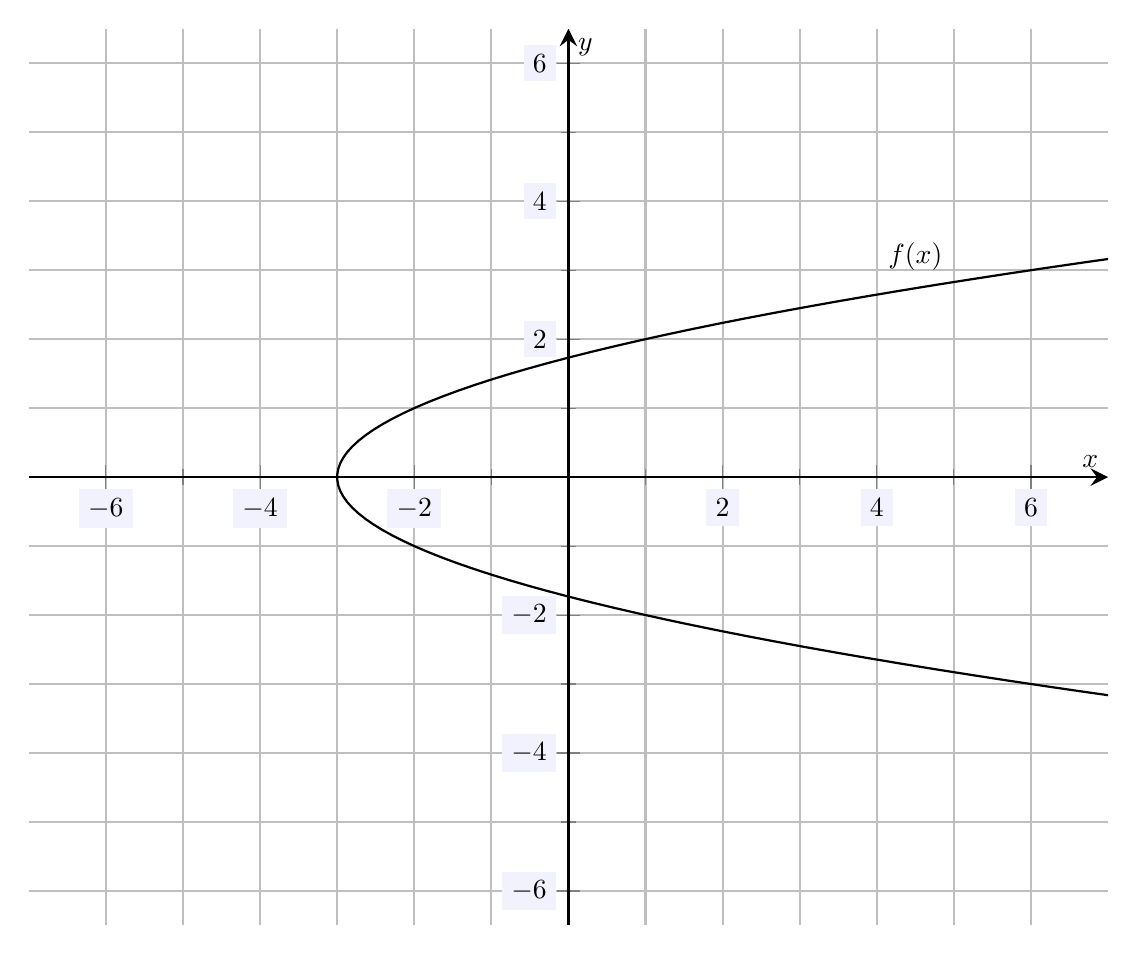
\begin{tikzpicture}[scale=2,every node/.style={scale=0.5}]
	\begin{axis}[
	grid=both,
	axis lines=middle,
	ticklabel style={fill=blue!5!white},
	xmin= -7, xmax=7,
	ymin= -6.5, ymax=6.5,
	xtick={-6,-4,-2,0,2,4,6},
	ytick={-6,-4,-2,0,2,4,6},
	minor tick = {-5,-3,...,5},
	xlabel=\(x\),ylabel=\(y\),
	]
	\node at (4.5,3.2) {$f(x)$};
	\addplot [domain= -4:4,samples=100] ({x^2 - 3},{x}); 
	\end{axis}
	\end{tikzpicture}
	}
	\] \pspace

\begin{parts}
\item Is the relation plotted above a function? Explain. \pvspace{1cm}

{\itshape The relation $f(x)$ above is not a function because it fails the vertical line test.} \pvspace{2.4cm}

\item Does the relation above have an inverse function? Explain. \pvspace{1cm}

{\itshape The relation $f(x)$ above has an inverse function because it passes the horizontal line test.}
\end{parts}



\newpage



% Question 13
\question[10] Consider the functions given in the table below.
        \begin{table}[!ht]
        \centering
        \begin{tabular}{| c || c | c | c | c | c |} \hline
	$x$ & $0$ & $1$ & $2$ & $3$ & $4$ \\ \hline
	$f(x)$ & $1$ & $4$ & $0$ & $-2$ & $6$ \\ \hline
	$g(x)$ & $2$ & $3$ & $5$ & $\phantom{-}5$ & $7$ \\ \hline
        \end{tabular}
        \end{table}

Compute the following: \pspace
        \begin{enumerate}[(a)]
        \item $g(3)= 5$ \vfill
        \item $g(2) - f(3)= 5 - (-2)= 5 + 2= 7$ \vfill
        \item $f(0)\,g(1)= 1 \cdot 3= 3$ \vfill
        \item $(f + g)(4)= f(4) + g(4)= 6 + 7= 13$ \vfill
        \item $(f \circ g)(1)= f(g(1))= f(3)= -2$ \vfill
        \item $(g \circ f)(1)= g(f(1))= g(4)= 7$ \vfill
        \item $x$-intercept of $f(x)$: $(2, 0)$ \vfill
        \item $y$-intercept of $g(x)$: $(0, 2)$ \vfill
        \end{enumerate}



\newpage



% Question 14
\question[8] Find the equation of the line shown below:
	\[
	\fbox{
	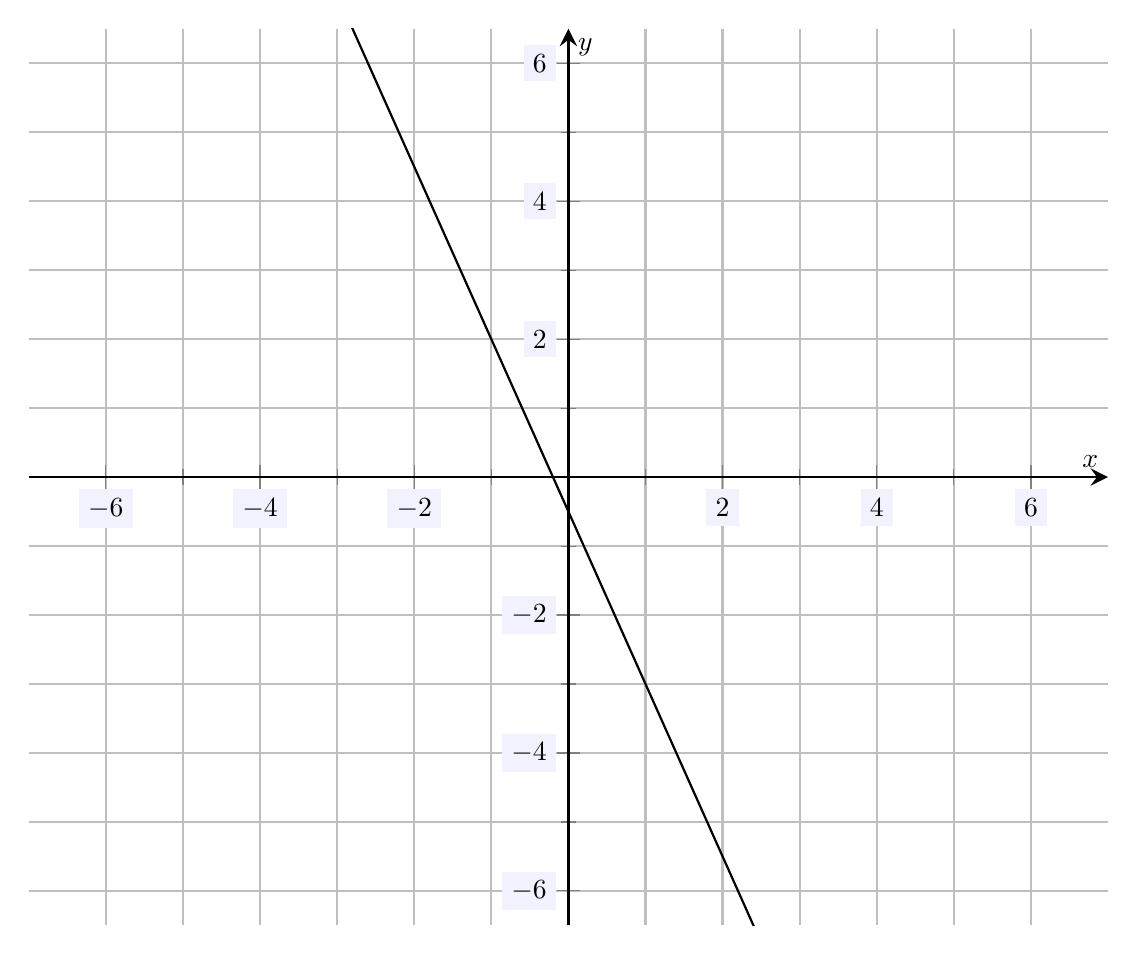
\begin{tikzpicture}[scale=2,every node/.style={scale=0.5}]
	\begin{axis}[
	grid=both,
	axis lines=middle,
	ticklabel style={fill=blue!5!white},
	xmin= -7, xmax=7,
	ymin= -6.5, ymax=6.5,
	xtick={-6,-4,-2,0,2,4,6},
	ytick={-6,-4,-2,0,2,4,6},
	minor tick = {-5,-3,...,5},
	xlabel=\(x\),ylabel=\(y\),
	]
	\addplot [domain= -4:4,samples=100] ({x},{-5/2*x - 1/2}); 
	\end{axis}
	\end{tikzpicture}
	}
	\] 

{\itshape The line is not vertical so that it has the form $y= mx + b$. The line passes through the point $(-1, 2)$ and $(1, -3)$. But then the slope is\dots
	\[
	m= \dfrac{2 - (-3)}{-1 - 1}= \dfrac{2 + 3}{-1 - 1}= \dfrac{5}{-2}= -\dfrac{5}{2}
	\]
Then we know $y= -\frac{5}{2}x + b$. But the line passes through the point $(-1, 2$), i.e. contains the point where $x= -1$ and $y= 2$, so that\dots
	\[
	\begin{aligned}
	y&= -\dfrac{5}{2}x + b \\
	2&= -\dfrac{5}{2} \cdot -1 + b \\
	2&= \dfrac{5}{2} + b \\
	b&= 2 - \dfrac{5}{2} \\
	b&= \dfrac{4}{2} - \dfrac{5}{2} \\
	b&= -\dfrac{1}{2}
	\end{aligned}
	\]
But then the equation of the line is $y= -\frac{5}{2}x - \frac{1}{2}$. 
}



\newpage



% Question 15
\question[8] Find the equation of the line that is perpendicular to the line $y= \frac{1}{2}\,x + 1$ that passes through the point $(2, 1)$. \pvspace{0.3cm}

{\itshape The line $y= \frac{1}{2}\,x + 1$ is not horizontal so that a line perpendicular to it will not be vertical. Then our line must have the form $y= mx + b$. Because the line is perpendicular to the line $y= \frac{1}{2}\,x + 1$, the slope of our line is the negative reciprocal of the slope of the line $y= \frac{1}{2}\,x + 1$. The slope of the line $y= \frac{1}{2}\,x + 1$ is $\frac{1}{2}$, so the slope of our line is $-\frac{2}{1}= -2$, i.e. $m= -2$. Then we know $y= -2x + b$. But the line contains the point $(2, 1)$, i.e. the point where $x= 2$ and $y= 1$. But then
	\[
	\begin{aligned}
	y&= -2x + b \\
	1&= -2(2) + b \\
	1&= -4 + b \\
	b&= 5 
	\end{aligned}
	\]
Therefore, the equation of the line is $y= -2x + 5$. 
}






\end{questions}
\end{document}